\documentclass[12pt]{article}
\usepackage{graphicx}
\usepackage{amsmath, amsthm, amssymb, amsbsy}
\usepackage[round]{natbib}
\usepackage{fourier}
\usepackage{setspace}
\usepackage{caption}
\usepackage{subcaption}
\usepackage{appendix}
\usepackage{threeparttable}
\usepackage{makecell}
\usepackage{placeins}
\usepackage{lscape}
\usepackage{tikz}
\usepackage{enumitem}
\usepackage{floatpag} %lets you turn off page number on the float page with \thisfloatpagestyle{empty}
\usepackage[capposition=top]{floatrow}
\usepackage{booktabs}
\usepackage[margin=1in]{geometry}
\usepackage{comment}
\usepackage[capposition=top]{floatrow}
\theoremstyle{definition}
\newtheorem{definition}{Definition}
%\usepackage[usenames,dvipsnames,svgnames,table]{xcolor}
\usepackage{xcolor}
\definecolor{olive}{rgb}{0.5, 0.5, 0.0}
\definecolor{midnightblue}{rgb}{0.1, 0.1, 0.44}
\definecolor{mediumelectricblue}{rgb}{0.01, 0.31, 0.59}
\definecolor{navyblue}{rgb}{0.0, 0.0, 0.5}
\usepackage{url}
\usepackage{color, colortbl, xcolor}
\usepackage{multirow}
\urlstyle{same} % Makes the font same as the surrounding text
\usepackage[colorlinks=true,
 			linkcolor=olive,
 			urlcolor=mediumelectricblue,
 			citecolor=mediumelectricblue
    ]{hyperref}
\definecolor{lg}{RGB}{245, 245, 245}

\newtheorem{theorem}{Theorem}
\newtheorem{assumption}{Assumption}
\newtheorem{proposition}{Proposition}

% For commenting
\newcommand{\tc}{\textcolor}
\newcommand{\MM}[1]{\textcolor{violet}{[ML: #1]}}
\newcommand{\AM}[1]{\textcolor{teal}{[AM: #1]}}

\onehalfspacing

\begin{document}

%%%%%%%%%%%%%%%%%%%%%%%%%%%%%%%%%%%%%%%%%%%%%%%%
%%%%%%%%%%%%%%%%%%%% TITLE PAGE %%%%%%%%%%%%%%%%%%%%%
%%%%%%%%%%%%%%%%%%%%%%%%%%%%%%%%%%%%%%%%%%%%%%%%

\title{{Gambling with money you don't have: Credit cards, frictions and online sports betting}\thanks{We thank Greg Kaplan, Gianni La Cava, and seminar participants at the e61 Institute, and the 2025 Workshop of the Australian Macroeconomic Society for helpful comments and suggestions. }
}
\author{Aditya Maitra
\thanks{e61 Institute,
\href{mailto:adit.maitra@e61.in}{adit.maitra@e61.in}.}
\and \hspace{-0.1in} Matthew Maltman% 
\thanks{e61 Institute \& Kenneth C. Griffin Department of Economics, University of Chiacago, \href{mailto:matthew.maltman@e61.in}{matthew.maltman@e61.in}.~}
}
\date{\today \\ \textcolor{mediumelectricblue}{Preliminary and incomplete - please do not circulate} \\}

\maketitle
\vspace{-0.3in}
\begin{abstract} 
\noindent
% 100 words
\noindent Governments increasingly regulate sin goods by restricting the payment mechanisms through which they can be purchased, rather than directly taxing or limiting consumption. Using bank transaction data, we evaluate one such policy, Australia's 2024 ban on credit cards for online wagering. The ban reduced gambling, cutting participation among affected individuals by 10 to 15 per cent, but the response was self-selecting: the third of affected gamblers who quit were small, financially secure bettors, while intensive gamblers switched funding sources and continued. A simple model of payment choice reconciles the evidence and shows how delinking credit from gambling can reduce participation through payment frictions, while disproportionately affecting the users regulators may be least concerned about.
\\\\

\noindent\textbf{JEL Classification:} C51, D12, H22, L71, Q35, Q58 \\
\noindent\textbf{Keywords:} Sports Betting, Gambling, Frictions, Household Finance, Targeting.
\thispagestyle{empty}
\end{abstract}



\clearpage
\newpage
\onehalfspacing
\setcounter{page}{1}

\newpage

\section{Introduction}\label{intro}
Gambling markets around the developed world are growing rapidly in size and scope. In recent years, technological and regulatory changes have made it easier than ever before to place a bet, whilst simultaneously the expansion of consumer credit has made it easier than ever to fund one. As the size of these markets have grown, there has been growing attention from policy-makers, researchers, and the wider public on the harms associated with gambling. 

A common policy response across jurisdictions has been to restrict the paument mechanisms through which gambling can be funded, and in particular to sever the link between credit and wagering.%
    \footnote{The United Kingdom banned credit card gambling in 2020. Ireland's Gambling Regulation Act 2024 prohibits credit cards, credit facilities, and credit-loaded wallet payments at licensed operators. Australia extended its long-standing in-person credit card prohibition to online wagering in June 2024. In the United States, many states that have legalised online sports betting have simultaneously barred credit card deposits into wagering accounts, and twenty-two states and the District of Columbia prohibit credit card purchases of lottery tickets — a product those same governments sell.}
The rationale for these restrictions rests on two assumptions about the role of credit in gambling.First that those who gamble using credit are a more vulnerable population than other gamblers - less liquid, more indebted, and closer to financial distress. Second that access to credit casuies counterfactually worse outcomes for these individuals, enabling exzpenditure that liquid funds would alone would constrain and coverting gambling losses into high-interest debt.

Despite their growing prevalence, we have limited evidence on how these payment restrictions operate or whom they affect. A key constraint is data. Evaluating a payment restriction requires observing the same individual's payment behaviour and consumption jointly, at high frequency, across the period spanning the policy change — and specifically requires seeing not just that a person gambled, but which account funded the bet, and what happened to their behaviour when that funding source was restricted. Survey data and aggregate statistics cannot provide this. The absence of evidence has not, however, slowed the instrument's spread. Payment restrictions are now jumping beyond gambling: the United Kingdom's Financial Conduct Authority has recently proposed prohibiting retail consumers from using borrowed funds to purchase cryptoassets, citing concerns about unsustainable debt among a population whose credit-funded crypto purchases more than doubled in two years. The question of how these restrictions operate and for whom is becoming more pressing precisely as the evidence base remains thin.

This paper studies the incidence and effects of payment restrictions using Australia's 2024 ban on credit card deposits into online sports betting accounts as our environment. The ban prohibited wagering firms from accepting credit card payments, with compliance immediate and complete. The stated rationale was that credit access enables gambling that liquid funds would otherwise constrain, while exposing consumers to debt. Announcing the ban, the responsible minister argued that ``people should not be betting with money they don't have'' \citep{Rowland_credit_cards_ban_2024}.

Our evidence comes from consented, de-identified bank transaction data that link each individual's credit cards, transaction accounts, and wallet-routed payments, allowing us to observe the funding source behind every wagering deposit and substitution across accounts when one is removed. Australia provides a near-ideal setting for this question. Australians lose more to gambling per capita than any other population \citep{Peake2025_biggest_losers}. Sports betting has been legal since 1983 and federally regulated online since 2001, meaning ours is a mature market near its long-run equilibrium. The responses we measure therefore come from established consumers rather than from a market still adjusting to legalisation — the relevant benchmark for jurisdictions whose newly legal markets are heading toward maturity.

We identify three lessons from the Australian policy change. The first concerns the mechanics of how such restrictions bind. The fungibility of money means that payment restrictions are enforceable — compliance here was complete and immediate — but not necessarily binding in the way their rationale assumes. In our setting, gamblers could preserve access to credit by transferring funds from a credit card to a transaction account before depositing, at literally unchanged financial cost, since card-funded gambling was already treated as a cash advance by Australian banks. A credit card ban therefore does not sever the credit line; it moves it one step away. What survives of the policy is not a credit constraint but a convenience friction — the cost of reorganising payment routines — and the evidence is consistent with it being the friction, rather than any binding constraint, that drove behavioural change.

The raw data provide evidence on this mechanism. At the effective date, credit card–funded sports betting falls to zero, while wagering funded from transaction accounts increases. Because this substitution is only partial, total wagering among treated gamblers also declines (Figure \ref{rawdata}).

\begin{figure}[H]
    \centering
    \caption{Raw data on the policy response}
    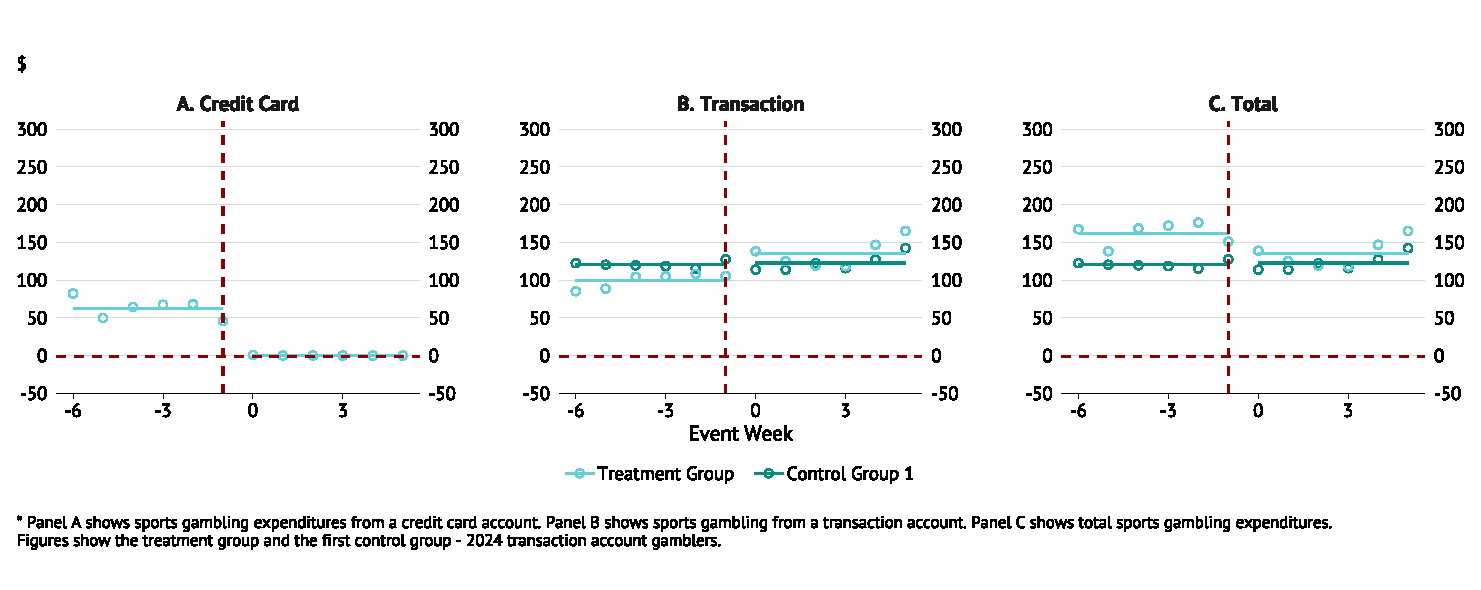
\includegraphics[width=\textwidth]{Figures/f5_raw_data.pdf}
    \label{rawdata}
\end{figure}

The second lesson concerns who these policies reach. Because access to credit is itself determined by private credit markets — which screen on financial standing, not on gambling behaviour — the population exposed to a credit payment restriction is not a random draw from the broader gambling market. In our data, gamblers who funded bets with a credit card had higher incomes and more liquid wealth than other gamblers, were no more likely to revolve credit card debt or face liquidity constraints, and funded most of their wagering from transaction accounts anyway. The composition premise underlying these policies fails: rather than reaching a more financially vulnerable population, the restriction hit those the private credit market had already screened toward financial health. This is not specific to Australia — it is a general property of restricting a screened instrument, and implies that the same restriction applied to a more lightly screened payment mechanism would reach a very different population.

The third lesson concerns how the friction affects the population it reaches. We find that gambling falls on average — total sports betting among treated individuals declined by around \$50 per fortnight — but the response is concentrated at the extensive margin, with the probability of wagering falling by 10 to 15 per cent while spending conditional on participating was unchanged. Critically, this participation decline is driven by a subset of gamblers who stopped entirely following the ban. These stoppers were disproportionately casual: they gambled less frequently and in smaller amounts before the ban, and were more reliant on the credit card as their sole funding source. The most heavily attached gamblers — those the policy was most concerned about — were the least likely to stop. The incidence of the friction is therefore governed by self-selection, and for a temptation good that selection runs in the wrong direction: willingness to step around a small hurdle rises with attachment to the activity, meaning frictions of this kind trim the casual edge of a market while leaving its core largely untouched.

%The remainder of the paper is structured as follows. Section \ref{sec:data} describes the institutional context, our data, and develops a conceptual framework that formalises the three lessons and generates testable predictions. Section \ref{sec:results} presents the empirical analysis. Section \ref{sec:conclusion} concludes.

\subsubsection*{Related literature}
This paper contributes to three strands of literature. The first is the long-standing debate on the effects of consumer credit access on household welfare. A large literature on payday lending and credit card contracts has examined whether expanded credit access helps or harms borrowers \citep[e.g.][]{melzer2011, morse2011, zinman2010, heidhues2010}. We bring this question to temptation goods, where the policy motivation is sharpest, and provide transaction-level identification of both who uses credit in such markets and what its removal does to their behaviour. The second is the behavioural public economics literature on corrective policy for goods with internalities. This literature has studied sin taxes \citep{allcott2019} and ordeal mechanisms as targeting devices for transfer programmes \citep{nichols1982, deshpande2019, thaler2018}. We contribute the first causal evidence on the incidence of a payment restriction aimed at a sin good, and show that the self-selection logic that makes ordeals useful for transfers runs in the opposite direction in temptation markets. The third strand is the growing literature measuring gambling behaviour and its consequences in financial transaction data \citep{muggleton2021, zendle2024}. Recent work using quasi-experimental variation in US legalisation has documented negative effects of sports betting access on household finances \citep{hollenbeck2025, baker2024}. We study the reverse experiment — an attempted contraction of access in a mature market — and examine whether the policy instrument used achieved its stated aims.

\section{Context}
\subsection{Policy context}
%\begin{itemize}
%    \item \AM{Details on policy change and it's motivation}
%    \item \AM{Details on implementation and effects}
%    \item \AM{Details on circumvention - explain here how people can transfer money across accounts and how the price of doing so is unchanged, but effort is.}
%\end{itemize}

Australia prohibited credit cards for in-person gambling in 2006, but online wagering, regulated federally since 2001, remained exempt. As online sports betting and its advertising grew, parliamentary inquiries recommended aligning the two regimes while acknowledging that evidence on the prevalence and harm of card-funded gambling was thin \citepalias{RegulationUseFinancialServicesOnlineGamblingAus}. On 7 December 2023 the Australian Federal Government announced the ban, which then took effect on 11 June 2024. The policy places the compliance burden on wagering firms, which must block deposits originating from credit cards, including card-funded deposits routed through digital wallets such as PayPal. Online lotteries were exempt. Firms complied completely and immediately: card-funded sports betting in our data falls to zero at the effective date (Figure \ref{rawdata}).


A key institutional feature of the Australian payments system is that banks classify gambling transactions made with a credit card as cash advances rather than purchases. Cash advances typically incur an upfront fee of around 3 per cent (or a \$3 minimum), accrue interest immediately without a grace period, and are subject to higher interest rates than ordinary purchases. Using a credit card to fund gambling was therefore already substantially more expensive than using a transaction account prior to the ban.

The same institutional arrangement also created a straightforward means of circumventing the policy. Rather than depositing directly with a credit card, a gambler could first transfer funds from the credit card into their transaction account and then deposit from that account. Because the initial transfer is also treated as a cash advance, this workaround carries essentially the same financial cost as a direct credit card deposit. The ban therefore did not increase the monetary cost of gambling on credit; instead, it introduced an additional step into the payment process. Gamblers who valued access to credit could continue borrowing at essentially unchanged cost, while those who used credit cards primarily for convenience would incur the cash advance fee without any corresponding benefit.



\subsection{Conceptual framework}\label{sec:model}
%\begin{itemize}
%    \item \AM{Details on how the ban binds and mechanical incidence. Explanation of how people can circumvent if needed.}
%    \item \AM{Model with heterogeneous types and two payment types. The model should do the following:}
%    \item \AM{Generate the composition prediction - screening means the two channel population differs from the one channel population.}
%    \item \AM{Generate the selection prediction - removing a channel produces exist concentrated among the low attatchment types.}
%    \item \AM{State the alternative predictions under the constraint mechanism so that we can compare the two - maybe?}
%\end{itemize}


To state ex ante what a payment friction should do to a market for a temptation good, we set out a simple model of payment choice with heterogeneous types. It has three ingredients: heterogeneity in the value gamblers place on wagering, a private market that screens access to one of two payment instruments on grounds unrelated to that value, and a one-off cost of switching instruments when one is withdrawn. Two predictions follow: one about who holds the instrument the policy will remove (composition), and one about who stops gambling once it is gone (selection).

\subsubsection*{Setup}

There is a unit mass of gamblers indexed by $i$, each described by a pair $(\theta_i, z_i)$. $\theta_i>0$ is $i$'s taste for gambling: the flow value derived from wagering each period, drawn from a distribution $F$ with full support. $z_i$ is a financial-standing variable -- income, liquid wealth, repayment history -- drawn from a distribution $G$. We do not restrict the joint distribution of $(\theta_i,z_i)$ beyond the screening assumption below; in particular, $\theta_i$ and $z_i$ need not be independent.

Each period a gambler funds wagers with one of two instruments, a transaction account $T$ or a credit card $C$. $T$ is available to everyone. $C$ is a screened product: $i$ holds a card if and only if $z_i\geq\bar z$, the threshold private lenders apply when underwriting cards. Let $a_i=\mathbf 1\{z_i\geq\bar z\}$ denote access.

\begin{assumption}[Screening on financial standing]\label{ass:screen}
Access is granted on $z_i$ alone: lenders underwrite credit cards on repayment risk, income, and financial history, not on gambling behaviour.
\end{assumption}

This is an institutional primitive rather than a result. It matches how consumer credit is priced in practice, and how credit-card holding in our data tracks income and liquid wealth rather than measures of gambling activity (Section~\ref{sec:data}).

Using the card carries a fee $f\geq0$ -- in our setting, the cash-advance charge on gambling deposits -- but yields a convenience benefit $c_i\geq0$ relative to the account: a single instrument to budget on, reward points, or habit. Flow utility from wagering with instrument $m\in\{T,C\}$ is
\begin{equation}\label{eq:flowutility}
u_{im} = \theta_i + \mathbf 1\{m=C\}\,(c_i-f).
\end{equation}
Convenience plausibly scales with how often a gambler tops up their wagering account, which rises with attachment, so we let $c_i=c(\theta_i)$ for a strictly increasing, continuous $c(\cdot)$.\footnote{Nothing below requires this monotonicity for the financial-composition result in Proposition~\ref{prop:composition}(a); it is what generates the taste-composition result in part (b).}

Among gamblers with access, $i$ uses the card if $c(\theta_i)\geq f$, i.e.\ if $\theta_i\geq\tilde\theta\equiv c^{-1}(f)$; gamblers with $a_i=1$ and $\theta_i<\tilde\theta$, and everyone with $a_i=0$, fund wagers from $T$. The population exposed to a ban on $C$ -- the treated group -- is
\begin{equation}\label{eq:treated}
\mathcal T=\{i: a_i=1 \text{ and } \theta_i\geq\tilde\theta\}.
\end{equation}

\subsubsection*{Composition}

\begin{proposition}[Composition]\label{prop:composition}
\begin{enumerate}[label=(\alph*)]
    \item \textbf{Financial composition.} $\mathcal T\subseteq\{i:z_i\geq\bar z\}$, so $E[z_i\mid i\in\mathcal T]\geq\bar z$. The treated population is at least as financially healthy as the credit-eligible population, and strictly healthier than the population of gamblers as a whole whenever $\bar z$ exceeds the population mean.
    \item \textbf{Taste composition.} $\mathcal T$ additionally requires $\theta_i\geq\tilde\theta$, so the distribution of $\theta$ in $\mathcal T$ is a right-truncation of $F$ at $\tilde\theta$. Under Assumption~\ref{ass:screen}, access does not select on taste, so $\mathcal T$ first-order stochastically dominates the population distribution of $\theta$: the treated group skews toward higher-taste gamblers than the average.
\end{enumerate}
\end{proposition}

Both parts share a source -- a threshold rule applied to a fixed population -- and together they say the group a payment ban exposes is not a random draw from the market: it is financially safer than average, screened on $z$, and simultaneously more attached to gambling than average, self-selected into card use on $\theta$. A policy premised on credit cards financing the most vulnerable or most indebted gamblers targets a group the private credit market has already screened away from that description.

\subsubsection*{Selection}

The ban withdraws $C$. A treated gambler who wants to keep gambling must re-register on $T$, paying a one-off switching cost $k_i\geq0$: linking a new account, moving auto-fill details, breaking a habit. Switching costs are naturally lower for gamblers who already used both instruments before the ban, since no new account or habit is required. With discount factor $\delta\in(0,1)$, gambler $i\in\mathcal T$ continues after the ban if and only if the continuation value exceeds the switching cost,
\begin{equation}\label{eq:continue}
\frac{\theta_i}{1-\delta}\geq k_i,
\end{equation}
and stops otherwise.

\begin{proposition}[Selection]\label{prop:selection}
Fix $k_i$. The probability of stopping is weakly decreasing in $\theta_i$: for any two treated gamblers with the same switching cost, the one with lower taste is weakly more likely to stop. If switching costs are lower for gamblers who used both instruments pre-ban, stopping is also decreasing in prior use of $T$.
\end{proposition}

\begin{proposition}[Irrelevance of financial standing within the treated group]\label{cor:z-irrelevant}
Conditional on $\theta_i$ and $k_i$, $z_i$ carries no additional information about stopping. Because $\mathcal T$ is already selected on $z_i\geq\bar z$ (Proposition~\ref{prop:composition}a), any remaining cross-sectional variation in continuation within $\mathcal T$ is driven by taste and switching cost, not by financial standing.
\end{proposition}

Proposition~\ref{prop:selection} is the model's selection prediction: exit concentrates among the low-taste, weakly attached members of the treated group, while funding wagers from both instruments pre-ban -- the empirical marker for a low switching cost -- predicts staying. Proposition~\ref{cor:z-irrelevant} is testable independently of it: liquidity, revolving status, and other markers of $z$ should not predict stopping once taste and prior instrument use are held fixed, not because financial standing is irrelevant to gambling in general, but because the treated sample has already been conditioned on it.

\subsubsection*{An alternative: the constraint model}

The model above treats the card as a convenience technology. An alternative, and the one motivating the policy, treats it as a source of credit: desired gambling is $g_i$, feasible gambling is $\min(g_i, w_i+L_i)$ for liquid wealth $w_i$ and credit line $L_i$, and the ban deletes $L_i$. This constraint model makes different predictions on both margins we study here. On composition, it predicts the treated group is the illiquid and indebted -- the opposite of Proposition~\ref{prop:composition}(a). On selection, it predicts compression among gamblers with $g_i>w_i$ regardless of taste, and it predicts financial improvement -- falling debt, rising balances -- among those who stop, neither of which is implied by Proposition~\ref{prop:selection}. The two models are therefore separable in the data, and we take each margin to the evidence in Section~\ref{sec:results}
\subsection{Data}
%\begin{itemize}
%    \item \AM{Bank transaction data information. Data source, what we observe.}
%    \item \AM{Measurement - Sample cleaning, Gambling transactions, other relevant information.}
%\end{itemize}
We use consented, de-identified bank transaction data collected by a third-party provider during routine consumer finance applications, including mortgages, credit cards, buy-now-pay-later products, personal finance apps, and utility switching. Each individual contributes a backward-looking window of financial history, typically 90 days of transactions across all linked accounts, covering spending, income, and balances on transaction, savings, and credit card products. The provider categorises transactions and strips personally identifiable information before we see the data. The source earns its place here by linking account types within a person, letting us attribute each wagering deposit to a funding source and watch activity move between accounts when the policy lands. We drop individuals with no observed credit card but with evidence of card use, such as card repayments leaving the transaction account, since we would otherwise misclassify them as non-cardholders.
 
We measure gambling as deposits into sports betting accounts, identified from merchant codes and verified against every major Australian operator. Sports betting is the dominant form of online gambling in Australia. Deposits track spending rather than losses, since we do not observe bets funded from a balance already sitting with the operator or from winnings left there. In-person betting, which Australians mostly conduct in cash, is invisible to us. We can however, test whether cash withdrawals increase after the policy, and find no evidence for this.\footnote{A note on Paypal and other third party intermediaries. Individuals may deposit funds into their sports betting account via PayPal. In this instance, the payment is initiated through PayPal, but the funds are drawn from their linked account. As a result, this activity appears in our data as a sports betting transaction from that account, and is therefore captured in our analysis. Note that the use of credit cards to deposit into sports betting accounts via PayPal was also prohibited under the policy. However, if an individual first deposits funds into their PayPal balance and subsequently uses those funds for gambling, we would not directly observe this activity in our data. To test whether this could be occurring, we also look at the effect of the policy on deposits into PayPal accounts around the policy implementation. We find no effect (Figure \ref{DiD_cash_paypal}}
 
Income is measured as regular, identifiable wage or income-support inflows. Expenditure is outlays on services and non-durables, with durables excluded so that lumpy purchases do not drive the series. We call someone liquidity constrained if their transaction balance falls below \$100 at any point in the pre-period, and a revolver if their outstanding card debt never falls below \$100.
 
The sample skews young and liquidity constrained relative to the population, due to the consumer-finance origin. The direction of the resulting bias is unclear: problematic gambling may concentrate among liquidity-constrained people, and the most problematic gamblers may also never appear in a finance application. Transaction data of this type track official aggregate consumption statistics closely in other work, which limits the concern.\CQ{cite the Australian benchmarking work here.} Benchmarking our card shares against public sources is harder, because little exists. Industry submissions put the credit card share of wagering deposits near 20 per cent in the late 2010s \citep{AustralianBankingAssociation2020UseCreditCardsGambling}, and TAB's chief executive reported 14 per cent in 2021, down from 15.7 per cent the year before \citepalias{RegulationUseFinancialServicesOnlineGamblingAus}. Our shares sit below that for two reasons: card use for gambling has fallen over time and our window is later, and card holding in our sample runs below the population rate. Conditional on holding a card, our card share of gambling is close to the industry figures (Online Appendix). The low card-holding rate does not threaten internal validity, provided the cardholders we observe resemble the ones we do not, in which case the response we estimate applies to card gamblers generally.




\section{Empirical analysis}
\subsection{Screening of the treated population}

Prior to the policy, credit cards represented only a minority, and a declining share, of the online sports betting market (Figure \ref{incidence}). In our data they funded 8 per cent of sports betting expenditure in late 2019, declining steadily to roughly 2 per cent in the months preceding the ban (Panel A). This decline is consistent with broader reductions in credit card use in Australia, particularly among younger cohorts, as well as industry testimony in 2021 reporting a decline in gambling funded by credit cards.\citepalias{RegulationUseFinancialServicesOnlineGamblingAus}. By early 2024, only 2 per cent of cardholders recorded any gambling from their card, and less than 10 per cent of card holders' gambling expenditure came from it. Any harms associated with credit card gambling were therefore already diminishing before the reform, although perhaps not zero.\footnote{The share of 25 to 34 year olds holding a credit card fell from 53 per cent in 2010 to 28 per cent in 2023. The only Australian survey to ask directly found 0.8 per cent of respondents reporting increased credit card debt from gambling in 2024 \citep{RockloffRussellBrowneHing2025}. In the HILDA survey, credit card ownership correlates positively with sports betting spending but negatively with problem gambling.}

Accounts using a credit card for sports gambling on average gambled more per week and carried more outstanding debt than other groups (Panel B), but these gaps reflect capacity rather than distress. Card gamblers had higher incomes and greater liquid wealth than their counterparts, were no more likely to revolve their credit card debt or face liquidity constraints, and funded a relatively large share of their weekly gambling from transaction accounts anyway (Panel C). This is consistent with the nature of credit card lending in Australia: credit cards are a screened product, issued only after lenders assess applicants' financial circumstances. The financially secure were disproportionately likely to hold the payment technology the ban removed.

Gambling among card users is also heavily right-skewed, ranging from roughly \$10 per week in the lowest quartile to \$600 in the highest. Yet even in the highest quartile, most gambling expenditure was funded from transaction accounts rather than credit cards, while measures of liquidity constraints and debt revolving show no clear differences across the distribution (Panel D). This makes it unlikely that access to short-term credit was driving large gambling expenditures. We cannot identify problem gambling directly, since doing so requires survey-based measures, and these averages do not rule out financial harm among some individuals in the group. But the typical card gambler was not in financial distress or using debt to finance gambling; for this group, credit cards appear to have served as much as a payment mechanism as a source of credit.

\begin{figure}[H]
    \centering
    \caption{Credit cards and sports betting before the ban}
    % TODO: current standalone charts dropped in as panels for now; recombine into a
    % single properly typeset 4-panel figure before submission, with notes carrying the
    % $100 constraint/revolver definitions and a shared group legend.
    \begin{subfigure}{0.49\textwidth}
        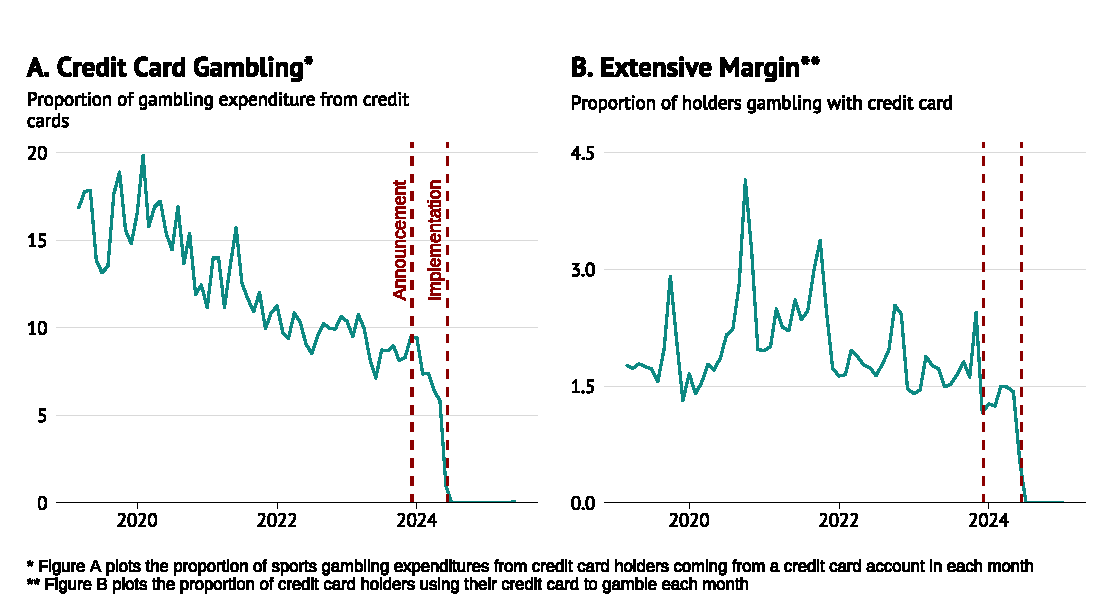
\includegraphics[width=\textwidth]{Figures/f1_timeseries_card_use.pdf}
        \caption{Card share of wagering over time}
    \end{subfigure}
    \begin{subfigure}{0.49\textwidth}
        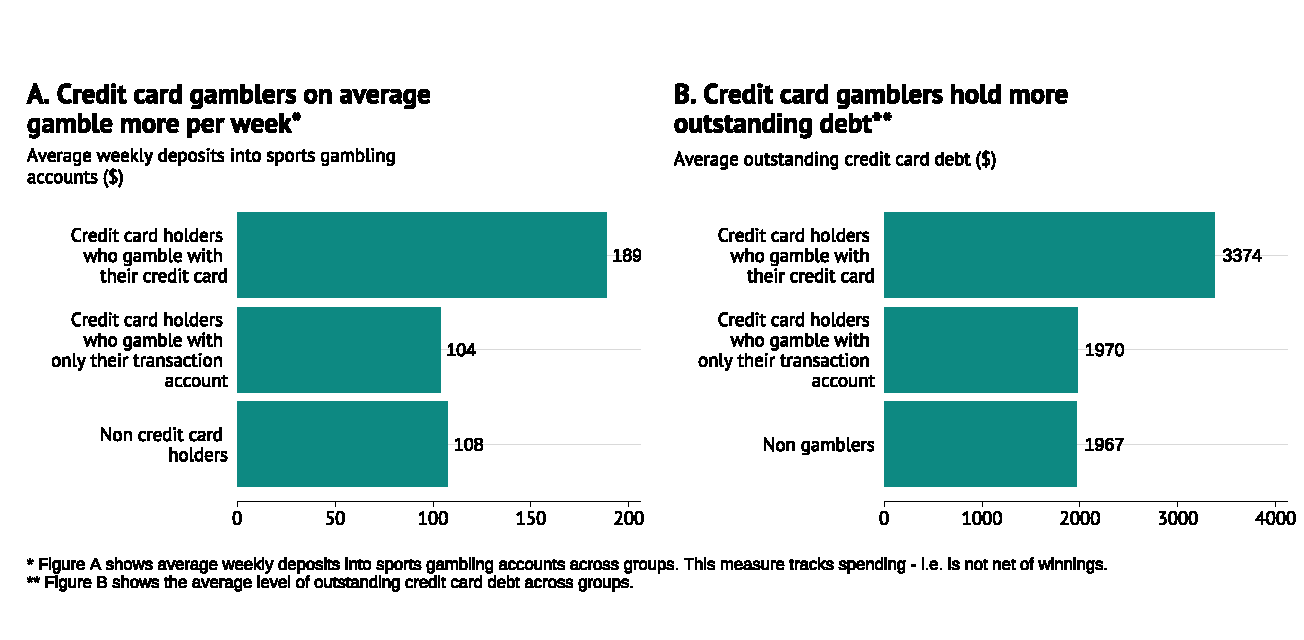
\includegraphics[width=\textwidth]{Figures/f2_gambling_creditdebt.pdf}
        \caption{Gambling and card debt across groups}
    \end{subfigure}
    \begin{subfigure}{0.49\textwidth}
        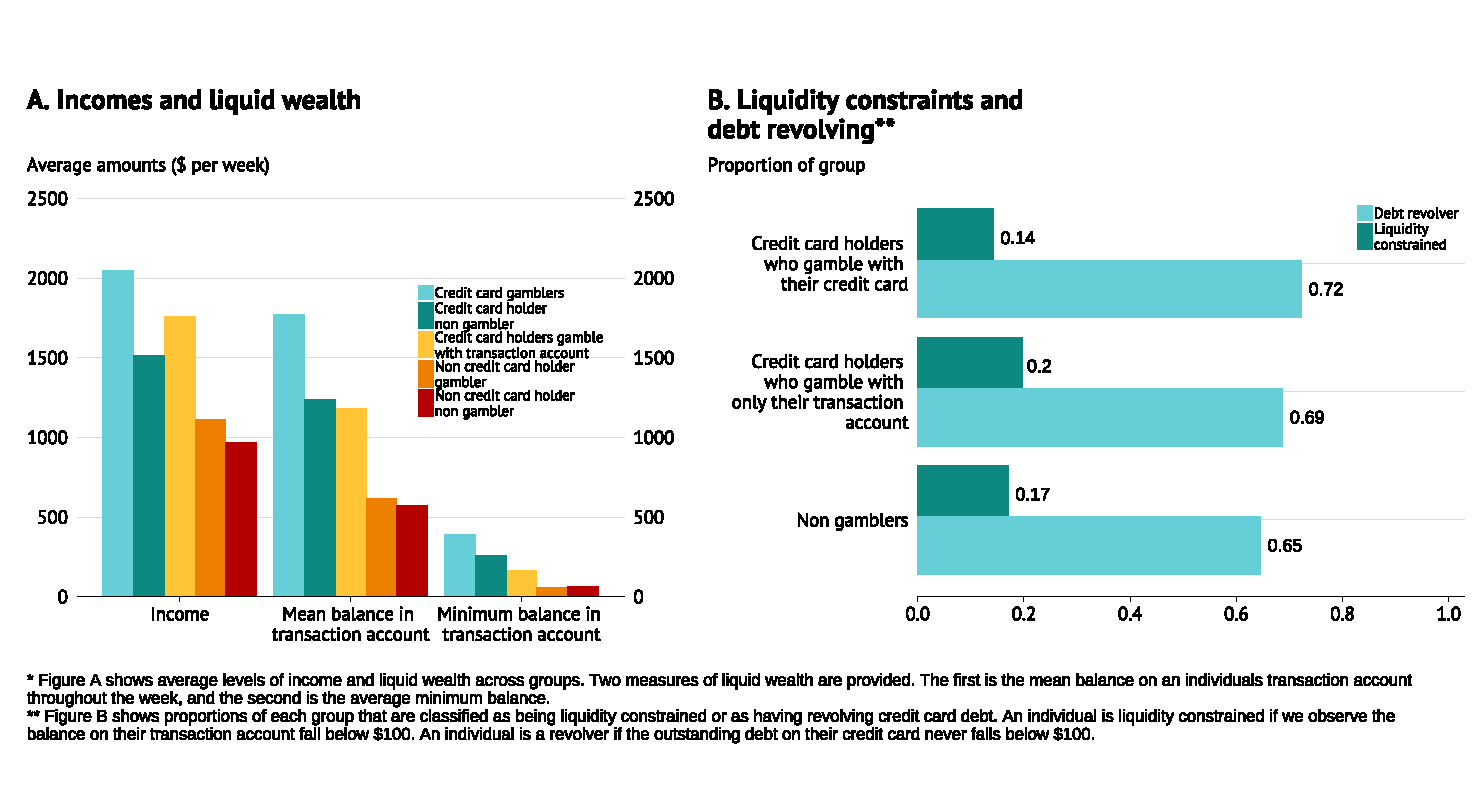
\includegraphics[width=\textwidth]{Figures/f3_income_wealth_lq.pdf}
        \caption{Income, liquid wealth, and constraints}
    \end{subfigure}
    \begin{subfigure}{0.49\textwidth}
        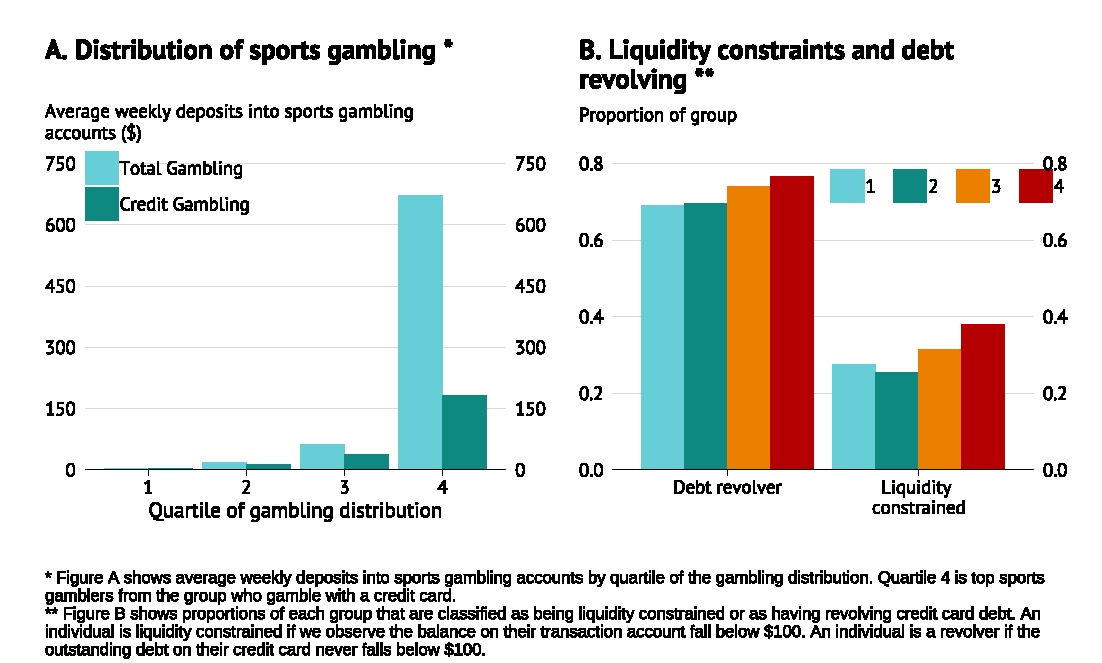
\includegraphics[width=\textwidth]{Figures/f4_gambling_right_skew.pdf}
        \caption{Outcomes across the card-gambler distribution}
    \end{subfigure}
    \label{incidence}
\end{figure}



\subsection{Econometric model}
%\begin{itemize}
%    \item \AM{Econometric framework with equation}
%    \item \AM{Identification: assumptions, threats and tests}
%\end{itemize}

We build a balanced fortnightly panel over a 20-week window spanning 4 April to 14 August in both 2023 and 2024, keeping individuals observed in each of the six weeks either side of the policy date, with at least one wage inflow per month, five expenditure outflows per month, and a sports gambling transaction before 11 June 2024. Our data are at the individual transaction level, but we aggregate to fortnightly to smooth idiosyncratic pay and betting cycles. Our results are robust to weekly frequency and to balanced windows of 4, 8, and 12 weeks around the treatment date (Online Appendix). The rolling structure of the data caps the horizon: we observe accounts for roughly 90 days on average, so beyond 12 weeks attrition dominates and the treated group shrinks.

We define treatment by pre-ban behaviour: individuals who funded sports gambling with a credit card at least once in 2024. We use two control groups: 2024 transaction-account gamblers, who held no credit card and were unaffected by the policy, controlling within-year for the sporting calendar; and 2023 credit card gamblers over the same calendar window, controlling across years for the behaviour of card gamblers absent the policy. Our baseline event-study specification is
\begin{equation}
    y_{it} = \alpha_i + \gamma_t + \textstyle\sum_t \beta_t \, (\text{Treat}_i \times F_t) + \epsilon_{it},
\end{equation}
with individual and period fixed effects, where outcomes are fortnightly sports gambling expenditure, an indicator for any gambling, gambling by funding instrument, non-gambling expenditure, balances, and fees.
Each control has limitations. Within-year comparisons may confound differential responsiveness to sporting events, and cross-year comparisons may confound differences in event calendars.\footnote{The 2023 window contained the Ashes and the FIFA Women's World Cup; the 2024 window contained the T20 World Cup and the UEFA European Championship.} 

We address this three ways. 
First, we estimate a triple-difference specification interacting year and card status. This specification uses differences between credit card and transaction-account gamblers within 2023 to absorb differential responses to sporting events, while differences between transaction-account gamblers in 2023 and 2024 absorb changes in the event calendar across years. The resulting estimates therefore more cleanly isolate the effect of the policy.
Second, because transaction-account gamblers on average gamble and earn less than treated individuals, we construct a nearest-neighbour matched sample, pairing each treated individual with the control gambler closest in pre-policy gambling expenditure and income. Third, we conduct placebo tests that reproduce the event-study specifications in settings where no policy change occurred: comparing credit card and transaction-account gamblers within 2023, and transaction-account gamblers across 2023 and 2024. Both placebo estimates are flat, while the triple-difference estimates closely track the baseline results (Online Appendix).


\subsection{Empirical results}
%\begin{itemize}
 %   \item \AM{(1) Aggregate fall in gambling with imperfect substitution. (2) Effects mainly driven by extensive margin. (3) EM mainly driven by group of stoppers who were more likely to be casually attached. (4) Other results - but keep this section brief.}
%\end{itemize}



We find the policy reduced average sports gambling among treated individuals by around \$50 per fortnight (Figure \ref{DiD}, Panel 1C), a result robust to the choice of control group, the triple difference, and the matched sample. Panels 1A and 1B decompose the response by funding source: credit card gambling falls mechanically to zero, by around \$100 per fortnight, and significant substitution to transaction accounts, of around \$50 per fortnight, which offsets around half of that fall.

The entire fall in spending is driven by the extensive margin, or participation: treated gamblers are 10 to 15 per cent less likely to wager in a given fortnight after the ban (Panel 2C), while the amount wagered conditional on gambling shows no change (Figure \ref{mechanisms}, Panel (b)).\footnote{All groups decline somewhat post-window by construction, since the sample conditions on pre-period gambling; we construct the control groups identically, so the event-study contrasts net this out. Average effects expressed in percentage changes are large, because casual gamblers with small baselines dominate the treated group (Online Appendix).} The extensive margin also shows the substitution, with the probability of gambling from a transaction account rising by roughly 10 per cent. In other words, the policy made treated accounts less likely to gamble at all rather than reducing betting amounts for those who kept gambling.

We also find no evidence of substitution into channels we cannot observe directly: in-person gambling requires cash and wallet-mediated gambling requires wallet deposits, yet neither cash withdrawals nor PayPal deposits move after the ban, and total online gambling including exempt lotteries falls in line with sports betting (Online Appendix).

Effects are also broadly consistent across the distribution of pre-treatment gambling. Pre-ban gambling among treated accounts ranges from roughly \$10 in the lowest quartile to approximately \$1,000 per fortnight in the highest; participation falls in every quartile, with larger proportional declines among those more casually attached to the market and mechanically larger dollar declines among high spenders given their higher baselines, and the extensive margin dominates everywhere. Splits by income, liquidity, constraint status, debt, and revolving show no meaningful heterogeneity (Online Appendix). Wherever we look, the ban removed gamblers rather than shrinking gambling.

\begin{figure}[H]
    \centering
    \caption{Event-study estimates of the policy response}
    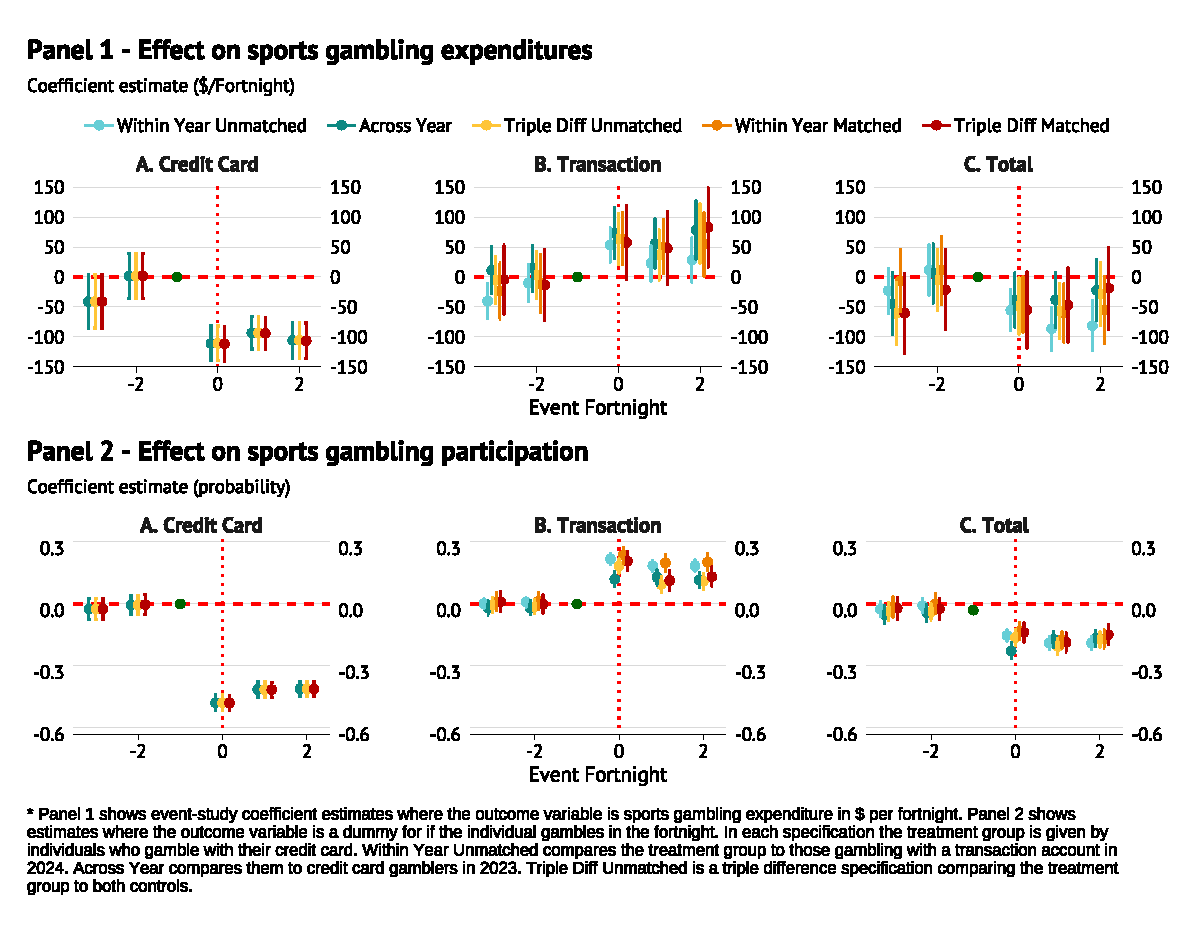
\includegraphics[width=\textwidth]{Figures/f6_DiD_baseline.pdf}
    \label{DiD}
\end{figure}

Reduced gambling did not visibly reappear as other spending or saving. Non-gambling expenditure shows no rise in the month after the ban, and transaction balances show little effect on their minimum, mean, or maximum. Credit card debt declines gradually over the three post-ban fortnights, by about \$500 on average and concentrated in the right tail, but the estimate is imprecise and not statistically significant. We therefore cannot conclude that the policy materially affected expenditure, savings, or debt in the short run. Mechanically, reduced gambling must translate into higher savings or other spending absent income changes, yet a \$50-per-fortnight effect is too small to generate detectable changes against normal week-to-week volatility within six weeks; longer-run accumulation of gambling savings remains possible but lies beyond our horizon. 

We aso find cash-advance fees on treated accounts fall by about \$4 per fortnight, and treated gamblers become around 30 per cent less likely to incur such a fee in a given fortnight, a transfer from banks to gamblers we return to below.


% TODO (extension): a sharper lottery test exists. Online lotteries were exempt, so
% card-funded lottery deposits among treated individuals should be UNCHANGED at the
% ban date. A within-person placebo validating merchant categorisation. One OA figure.

\subsection{Mechanisms}\label{sec:mechanisms}

We decompose the participation effect by splitting treated gamblers into \emph{stoppers}, who record no wagering in the six weeks after the ban, and \emph{switchers}, who continue from other accounts. Stoppers are 38 per cent of the group, and Panel (a) of Figure \ref{mechanisms} shows they drive essentially all of the participation effect: once an individual switches funding sources, their probability of gambling in a fortnight sits near the counterfactual. The policy cleaved off a group who never re-registered and barely touched everyone else. Their cessation looks real rather than incidental: 60 per cent of eventual stoppers gambled in any given fortnight before the policy, so recording nothing across the entire post-period suggests a meaningful medium-run effect at a minimum. Our six-week window cannot rule out an eventual return, a question we take up in Section \ref{Framework}. Nor can we observe which friction bound for whom: some stoppers may have lacked a debit card, others had never linked one to a wagering account, and others may have wanted to quit and treated the ban as the occasion.

\begin{figure}[H]
    \centering
    \caption{Decomposing the response}
    % TODO: current standalone charts dropped in as panels for now; recombine into a
    % single properly typeset 3-panel figure before submission.
    \begin{subfigure}{0.85\textwidth}
        \centering
        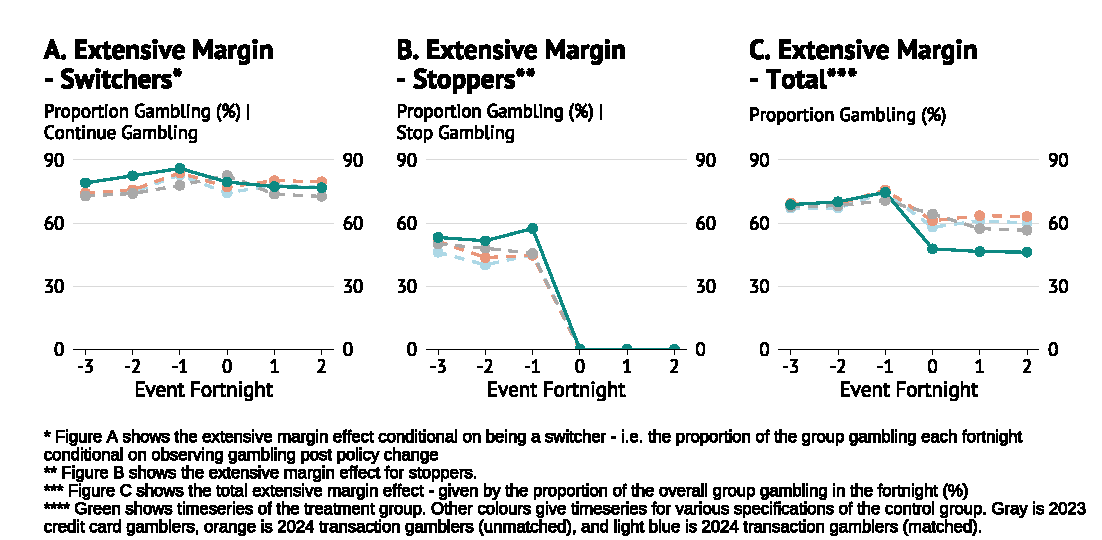
\includegraphics[width=\textwidth]{Figures/f9_stoppers_switchers.pdf}
        \caption{Stoppers versus switchers}
    \end{subfigure}\\
    \begin{subfigure}{0.85\textwidth}
        \centering
        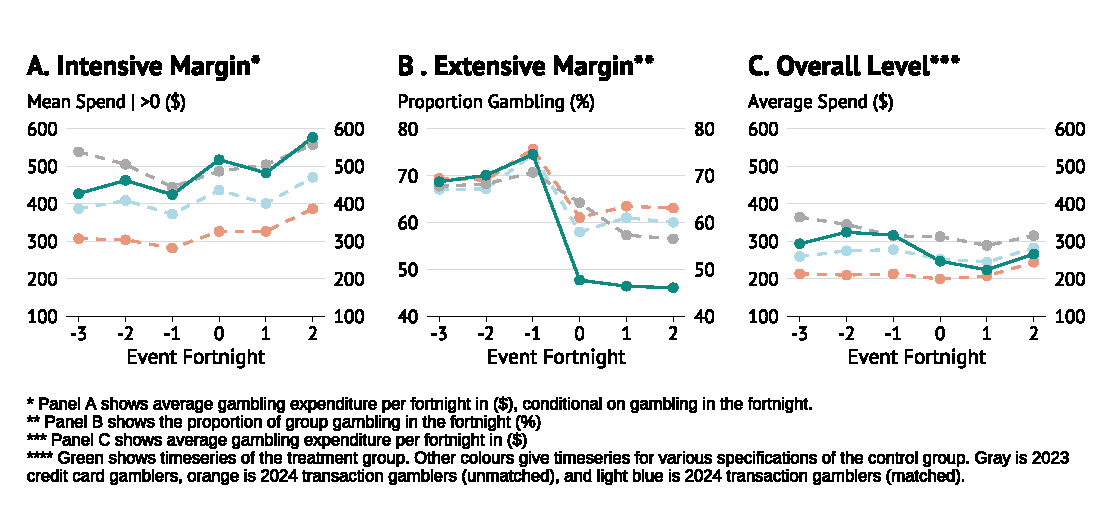
\includegraphics[width=\textwidth]{Figures/f7_EMIM_effects.pdf}
        \caption{Extensive versus intensive margins}
    \end{subfigure}\\
    \begin{subfigure}{0.85\textwidth}
        \centering
        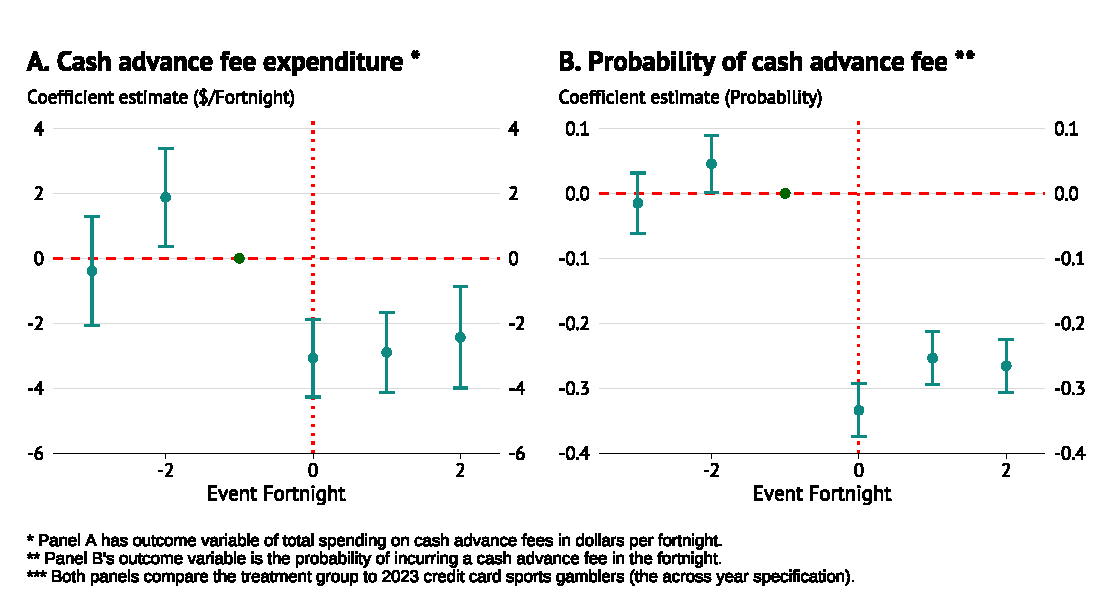
\includegraphics[width=\textwidth]{Figures/fB18_cash_advance_fees.pdf}
        \caption{Cash advance fees}
    \end{subfigure}
    \label{mechanisms}
\end{figure}

Two pre-ban characteristics predict who stops (Table \ref{tab:stoppers}). Gamblers in higher intensity quartiles are 10 to 22 percentage points less likely to stop than the lowest quartile, and gamblers who already funded wagers from both instruments are 44 percentage points less likely to stop than those reliant on the card alone. The variables a borrowing story nominates do nothing: liquidity constraint, revolving status, balances, and debt are precisely estimated zeros once we control for intensity and funding-source use. Attachment to the activity and exposure to the switching cost predict exit; financial position does not.

\begin{table}[!htbp]
\centering
\caption{Predictors of stopping after the ban}
\label{tab:stoppers}
\begin{adjustbox}{width=0.88\textwidth, center}
\begin{threeparttable}
\scriptsize
\begin{tabular}{@{\extracolsep{5pt}}lccccc}
\\[-1.8ex]\hline
\hline \\[-1.8ex]
 & (1) & (2) & (3) & (4) & (5) \\
\hline \\[-1.8ex]
\multicolumn{6}{l}{\textit{Dependent variable: Stopper (1 = no gambling in six weeks post ban)}} \\
\hline \\[-1.8ex]
Gambling Quartile 2  & $-$0.204$^{***}$ &  & $-$0.102$^{**}$ & $-$0.102$^{**}$ & $-$0.106$^{**}$ \\
 & (0.036) &  & (0.034) & (0.034) & (0.034) \\[0.4em]
Gambling Quartile 3 & $-$0.339$^{***}$ &  & $-$0.149$^{***}$ & $-$0.149$^{***}$ & $-$0.152$^{***}$ \\
 & (0.037) &  & (0.035) & (0.035) & (0.035) \\[0.4em]
Gambling Quartile 4 & $-$0.514$^{***}$ &  & $-$0.214$^{***}$ & $-$0.213$^{***}$ & $-$0.218$^{***}$ \\
 & (0.037) &  & (0.038) & (0.038) & (0.038) \\[0.4em]
Both accounts &  & $-$0.520$^{***}$ & $-$0.443$^{***}$ & $-$0.444$^{***}$ & $-$0.437$^{***}$ \\
 &  & (0.024) & (0.027) & (0.028) & (0.028) \\[0.4em]
Liquidity constrained &  &  &  & 0.006 &  \\
 &  &  &  & (0.026) &  \\[0.4em]
Revolver &  &  &  & 0.003 &  \\
 &  &  &  & (0.024) &  \\[0.4em]
Log(Transaction Balance) &  &  &  &  & 0.006 \\
 &  &  &  &  & (0.007) \\[0.4em]
Log(Credit Card Debt) &  &  &  &  & 0.003 \\
 &  &  &  &  & (0.010) \\[0.4em]
Constant & 0.663$^{***}$ & 0.651$^{***}$ & 0.729$^{***}$ & 0.726$^{***}$ & 0.659$^{***}$ \\
 & (0.026) & (0.017) & (0.024) & (0.028) & (0.094) \\[0.4em]
\hline \\[-1.8ex]
R$^{2}$ & 0.147 & 0.281 & 0.300 & 0.300 & 0.301 \\
\hline \\[-1.8ex]
\end{tabular}
\begin{tablenotes}
\item \textbf{Notes:} Linear probability models on the treated sample. Quartiles are of pre-ban fortnightly gambling expenditure. ``Both accounts'' indicates funding wagers from both a credit card and a transaction account pre-ban. Liquidity constrained: transaction balance falls below \$100 in the pre-period. Revolver: outstanding credit card debt never falls below \$100. Column (5) adds log mean pre-ban transaction balance and log mean credit card debt. Standard errors in parentheses. $^{*}$p$<$0.1; $^{**}$p$<$0.05; $^{***}$p$<$0.01.
\end{tablenotes}
\end{threeparttable}
\end{adjustbox}
\end{table}

The policy also never truly constrained the liquidity of card gamblers, because a simple workaround exists: transfer funds from the credit card to a transaction account, then deposit from there. This route incurs the same cash-advance fee that card gambling attracted before the ban, so a gambler who genuinely depended on card credit could have preserved their liquidity at essentially unchanged financial cost, and cash-advance fees should have remained steady after the policy. Instead they fall by roughly \$4 per fortnight among treated gamblers (Figure \ref{mechanisms}, Panel (c)): treated gamblers abandoned the credit channel rather than rerouting it. Financial outcomes agree. Stoppers and switchers show no differential movement in credit card debt or balances after the ban; only among top-quartile stoppers is there a suggestive decline in debt and rise in balances, imprecisely estimated on a small group, which is where any genuine constraint effect would live if one exists.


\section{Conclusion}
Payment restrictions have become the fashionable instrument of gambling regulation across the UK, the US, and Australia, justified as a curb on betting with borrowed money. Our evidence, from the first transaction-level evaluation of such a policy, is that the justification and the mechanism have little to do with one another. Credit card gamblers were financially secure consumers paying for convenience; removing their instrument imposed a small one-off friction; and that friction removed roughly a third of them, the most casual and the most reliant on a single payment mechanism, while the intensive core of the market switched instruments within a fortnight and carried on.

Read narrowly, this is an evaluation of one ban: effective at reducing participation, mistargeted relative to its stated aim, and modest in welfare terms either way. Read generally, it is evidence on how friction-based regulation of temptation goods works. Frictions move participation at trivial fiscal and political cost, which makes them genuinely valuable where the policy objective lives on the extensive margin, in immature markets or at the point of entry. But consumers set a friction's incidence when they decide whether to step around it, and for goods where attachment and harm travel together, that selection systematically spares the users policy is aimed at. Reaching them requires instruments that bind harder with intensity of use, not higher hurdles at the door.

\newpage
\bibliographystyle{apalike}
\bibliography{references}

\clearpage
\newpage

\appendix

% Page, figure, table, equation formatting
\renewcommand{\thepage}{A-\arabic{page}}
\renewcommand{\thefigure}{\thesection.\arabic{figure}} 
\renewcommand{\thetable}{\thesection.\arabic{table}} 
\renewcommand{\theequation}{\thesection.\arabic{equation}} 
\setcounter{page}{1}
\setcounter{figure}{0}
\setcounter{table}{0}
\setcounter{equation}{0}
\setcounter{footnote}{0}
\setlength{\abovedisplayskip}{2pt}
\setlength{\belowdisplayskip}{2pt}

\begin{center}
    \huge
    \textbf{Online Appendix}
\end{center}

\section{Robustness checks}\label{app:robustness}
\section{Additional results}\label{app:extra}


\end{document}
